\section{Auswertung}
\label{sec:Auswertung}

\subsection{Eichung des Elektromagnen}
\label{sec:Eichung}
Die Daten, die bei der Eichung des Magnetfeldes aufgenommen werden, sind
Abbildung \ref{fig:eichung} zu entnehmen. In dieser Abbildung ist zudem ein
Ausgleichspolynom dritten Gerades der Form
\begin{equation*}
  g(x) = a\cdot x^3 + b\cdot x^2 + c\cdot x + d
\end{equation*}
eingezeichnet. Dieses Polynom wird durch python/scipy berechnet \cite{scipy}.
Die aufgenommenen Werte sind lediglich darfür wichtig, dass das
möglichst optimale Magnetfeld anliegt um den Zeeman-Effekt beobachten zu können.
\begin{figure}
  \centering
  \includegraphics[width=\textwidth]{Eichung.pdf}
  \caption{Messwerte zur Eichung des Elektromagneten und das Ausgleichspolynom.}
  \label{fig:eichung}
\end{figure}

\subsection{Mögliche Übergänge um die blaue und rote Spektrallinie zu erzeugen}
\label{sec:Uebergaenge}
Für die rote Spektrallinie ($\lambda = 643.8\, \si{\nano\meter}$) der Cd-Lampe ist der Übergang
${^{1}P_\text{1} \leftrightarrow ^{1}D_\text{2}}$ verantwortlich. Die blaue
Spektrallinie ($\lambda = 480.0 \,\si{\nano\meter}$) wird durch den Übergang
${^{3}S_\text{1} \leftrightarrow ^{3}P_\text{1}}$ erzeugt. Aus dieser
Spektroskopischen Notation ergibt sich sofort:
\begin{align*}
  ^{1}P_\text{1} \rightarrow S=0, L=1, J=1\\
  ^{1}D_\text{2} \rightarrow S=0, L=2, J=2\\
  ^{3}S_\text{1} \rightarrow S=1, L=0, J=1\\
  ^{3}P_\text{1} \rightarrow S=1, L=0, J=1 .
\end{align*}
Der normale Zeeman-Effekt tritt bei der roten Linie auf. Bei dem normalen Zeeman-Effekt
ist der Landé-Faktor $g_\text{i}$ immer gleich eins. Bei dem anormalen Zeeman-Effekt
sind die Landé-Faktoren $g_\text{ij}$ verschieden. Für $^{3}S_\text{1}$ beträgt
$g = 2$ und für $^{3}P_\text{1}$ ist der Wert von $g = \frac{3}{2}$.

\subsection{Dispersionsgebiet und Auflösungsvermögen der Lummer-Gehrcke-Platte}
\label{sec:disp_aufl_lummer}
Das Dispersionsgebiet $\Delta \lambda_\text{D}$ der Lummer-Gehrcke-Platte
wird nach Gleichung \ref{eq:lambda_D} berechnet. Die in dieser Gleichung
vorkommende Dicke $d$ der Platte beträgt hier $d=4\,\si{\milli\meter}$.
Die Länge der Platte ist $L = 120 \,\si{\milli\meter}$. Der Brechungsindex $n$ ist
von der Wellenlänge des eingestrahlen Lichts abhängig:
\begin{align*}
  n(644\,\si{\nano\meter}) &= 1.4567\\
  n(480\,\si{\nano\meter}) &= 1.4635.
\end{align*}
Mit diesen Größen kann das Dispersionsgebiet berechnet werden zu:
\begin{equation}
  \label{eq:rot_Dispersionsg}
  \Delta \lambda_\text{D}(\lambda=643.8\,\si{\nano\meter}) = 48.913\,\si{\pico\meter}\\
\end{equation}
\begin{equation}
  \label{eq:blau_Dispersionsg}
  \Delta \lambda_\text{D}(\lambda=480.0\,\si{\nano\meter}) = 26.952\,\si{\pico\meter}.
\end{equation}
Das Auflösungsvermögen kann nach Gleichung \ref{eq:Aufloesung} berechnet werden.
Dabei ergeben sich nachfolgende Werte:
\begin{align}
  A(\lambda=643.8\,\si{\nano\meter})&=209063.644\\
  A(\lambda=480\,\si{\nano\meter})&=285458.063.
\end{align}

\subsection{Messung des Landé-Faktors}
\label{sec:Lande}
Um die aufgenommenen Bilder auszumessen und miteinander vergleichen zu können
werden die Bilder mit GIMP \cite{gimp} bearbeitet. Dazu wird der Bildteil, in welchem
das Interferenzmuster zu erkennen ist, ausgeschnitten und übereinander gelegt.
So kann entschieden werden, welche Linie in welche aufspaltet.
Als nächstes
werden die Positionen der Interferenzstreifen in Pixel ausgelesen und notiert.
Dabei wird nach Möglichkeit immer die Mitte, welche eine subjektive Auswahl ist,
der Interferrenz gemessen. Die Breite $\Delta s$ wird aus dem Bild ohne Einfluss
eines äußeren Magnetfelds ermittelt. Dazu werden die Abstände der benachbarten
Interferenzstreifen aus den Positionen bestimmt. Die Breite $\delta s$, welche
die Breite der Aufspaltung der Linien bei einem Magnetfeld angibt, wird ebenfalls
errechnet.
Aus den ausgemessenen Werten kann $\delta \lambda$ nach der Formel
\begin{equation}
  \label{eq:delta_lambda}
  \delta \lambda = \frac{1}{2} \frac{\delta s}{\Delta s}\cdot \Delta \lambda_\text{D}
\end{equation}
berechnet werden.
Zur Bestimmung der Landé-Faktoren wird die Gleichung \ref{eq:dE}
%\begin{equation}
%  | \Delta E | = | \Delta m | g \mu_\text{B} B
%\end{equation}
verwendet. In diesem Versuch ist $|\Delta m|$ immer gleich eins. %delta m kann doch auch 0 sein?
Außerdem ist die Gleichung $E=\frac{hc}{\lambda}$ gültig. Ableiten
dieser Gleichung ergibt:
\begin{equation}
 \frac{\partial E}{\partial \lambda} = -\frac{hc}{\lambda^2}\,\, .
\end{equation}
Somit ergibt sich:
\begin{equation}
 | \delta E | = \bigl| \frac{ch}{\lambda^2} \bigr| \cdot \delta \lambda \,\, .
\end{equation}
Durch Einsetzen von Gleichung \ref{eq:delta_lambda}
ergibt sich für die Berechnung des Landé-Faktors folgende Formel:
\begin{equation}
  \label{eq:Lande_berechnen}
 g = \frac{hc\cdot\delta\lambda}{\lambda^2\mu_\text{B}B}.
\end{equation}

\subsection{Für die rote Linie}
\label{sec:rot_Lande}
Das mit der Digitalkamera aufgenommene und zugeschnittene Interferenzbild
ist in Abbildung \ref{fig:rotcut} zu sehen.
Die sich bei der Berechnung nach Gleichung \ref{eq:delta_lambda}
ergebenden Werte für $\delta \lambda$ sind in Tabelle \ref{tab:rot_delta_s}
aufgelistet. Dabei wird für $\Delta \lambda_\text{D}$ der Wert aus \ref{eq:rot_Dispersionsg}
verwendet.
Die nach Gleichung \ref{eq:Lande_berechnen} berechneten Landé-Faktoren sind ebenfalls in Tabelle \ref{tab:rot_delta_s}
mit aufgelistet. Die dabei benötigte Planck Konstante beträgt $h =\SI{6.626e-34}{\joule\s}$ \cite{PlanckKonst},
die Lichtgeschwindigkeit beträgt $c=\SI{299792458}{\meter\per\s}$ \cite{Lichtgeschw} und das
Bohrsche Magneton beträgt $\SI{927.4e-26}{\joule\per\tesla}$ \cite{BohrMagneton}.
\begin{table}
  \centering
  \caption{Messwerte für die Ausmessung der roten Linie bei einem Magnetfeld von
  $B = \SI{638}{\milli\tesla}$. $\Delta s$ und $\delta s$ sind in Pixel angegeben.}
  \label{tab:rot_delta_s}
  \begin{tabular}{c | c | c | c}
    \toprule
    $\Delta s$ & $\delta s$ & $\delta \lambda \cdot 10^{-12}$ & $g$\\
    \midrule
    106.0 & 50.0 & 6.36 & 1.88 \\
    108.0 & 48.0 & 5.99 & 1.77 \\
    100.0 & 50.0 & 6.74 & 1.99 \\
    104.0 & 44.0 & 5.7 & 1.69 \\
    92.0 & 44.0 & 6.45 & 1.91 \\
    98.0 & 48.0 & 6.6 & 1.95 \\
    90.0 & 38.0 & 5.69 & 1.68 \\
    92.0 & 44.0 & 6.45 & 1.91 \\
    82.0 & 38.0 & 6.24 & 1.85 \\
    90.0 & 32.0 & 4.79 & 1.42 \\
    82.0 & 28.0 & 4.6 & 1.36 \\
    80.0 & 32.0 & 5.39 & 1.6 \\
    82.0 & 36.0 & 5.92 & 1.75 \\
    76.0 & 40.0 & 7.09 & 2.1 \\
    78.0 & 30.0 & 5.18 & 1.53 \\
    \bottomrule
  \end{tabular}
\end{table}
Es ergibt sich für den den Mittelwert des Landé-Faktor ein Wert von:
\begin{equation}
  \label{eq:lande_rot}
  g_\text{rot} = 0.995\pm0.018.
\end{equation}
Dieser Wert wird mittels python/numpy \cite{numpy} berechnet.
\begin{figure}
  \centering
  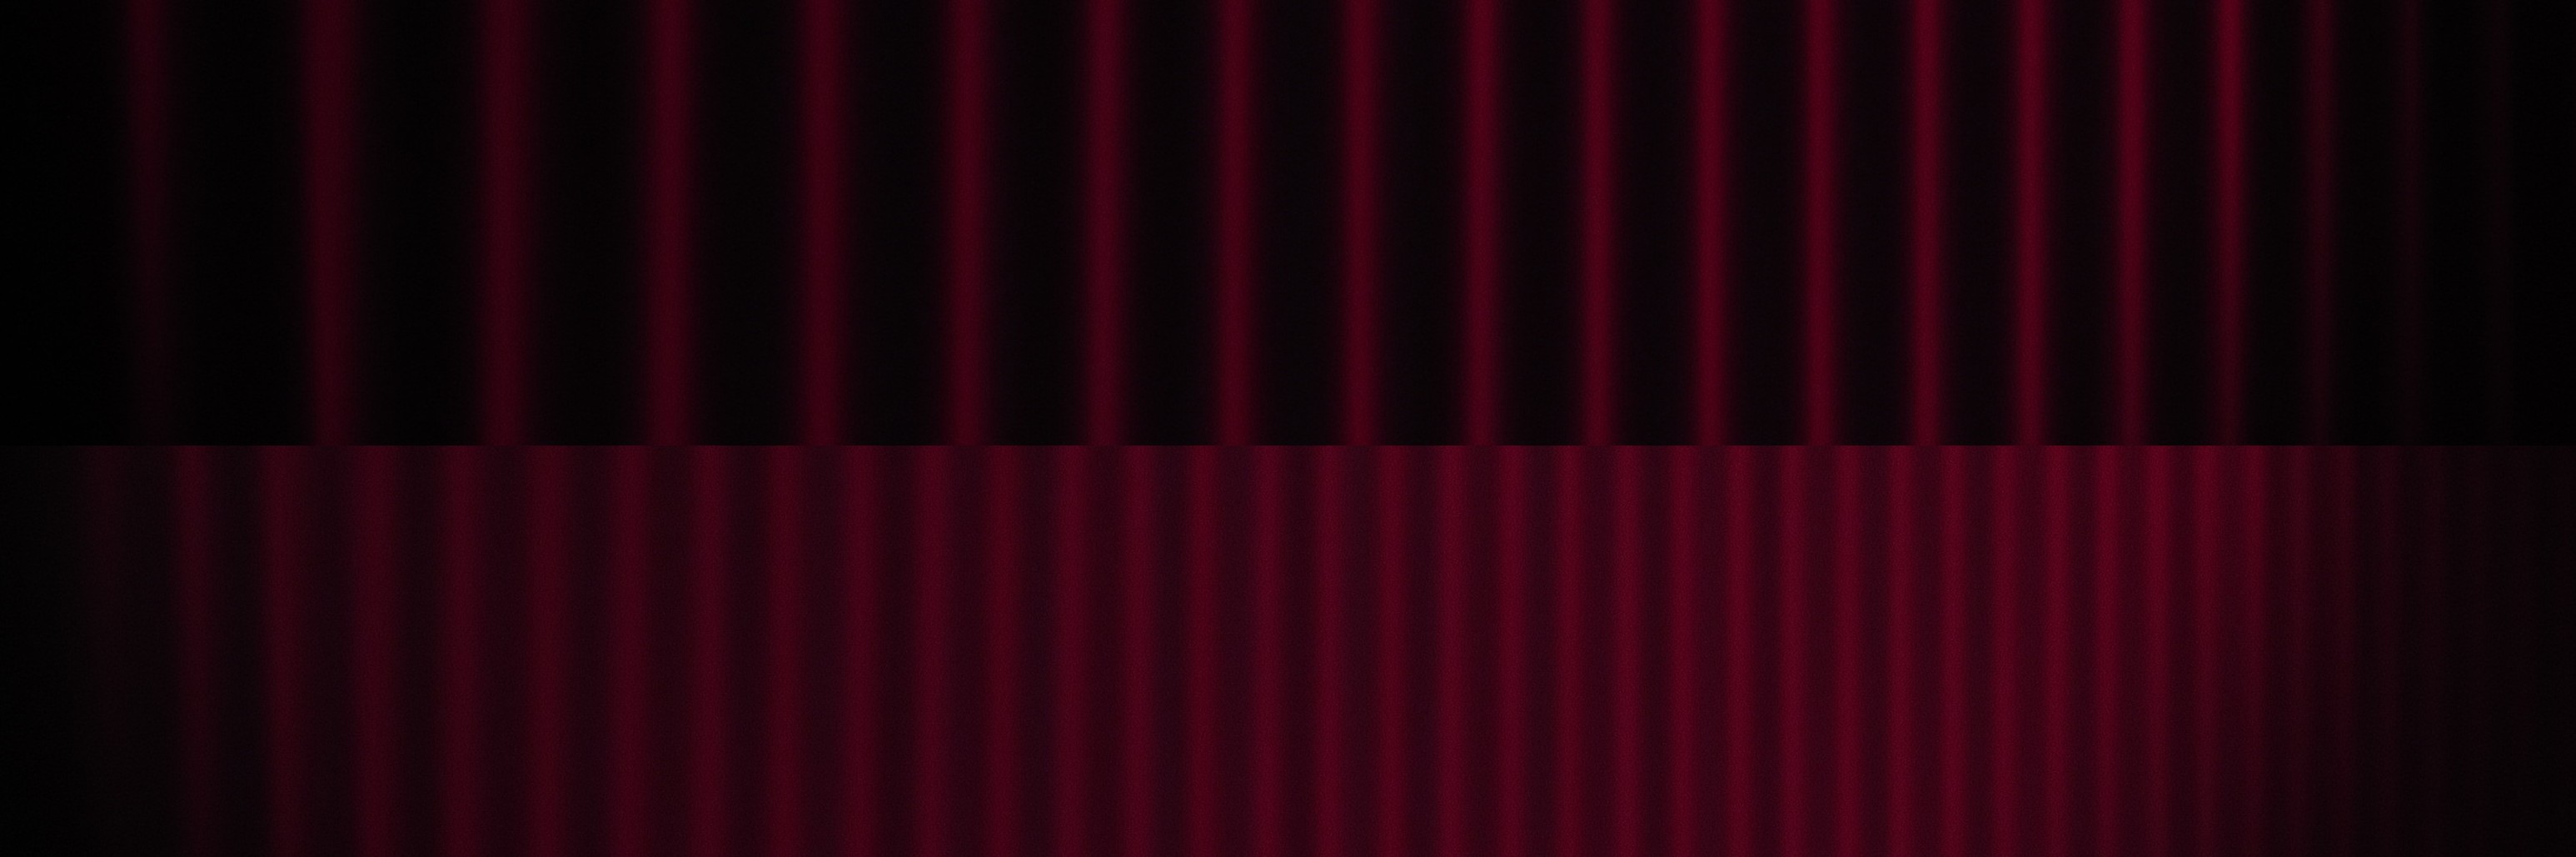
\includegraphics[width=\textwidth]{rotcut.jpg}
  \caption{Interferenzbild für die rote Linie. In der oberen Hälfte ist das Interferenzbild
  ohne ein äußeres Magnetfeld zu sehen. In der unteren Hälfte ist ein Magnetfeld von
  $B=\SI{638}{\milli\tesla}$ angelegt und der Polarisationsfilter auf $0°$ gestellt, sodass
  die $\sigma$-Polarisierung zu erkennen ist.}
  \label{fig:rotcut}
\end{figure}

\subsection{Für die Blaue Linie mit \texorpdfstring{$\pi$}{π}-Aufspaltung}
\label{sec:blau_pi_Lande}
Das sich bei der $\pi$-Aufspaltung der blauen Linie ergebende Interferenzbild
sowie das Interferenzbild ohne Magnetfeld sind in Abbildung \ref{fig:blaupicut}
zu sehen. Die sich bei der Berechnung ergebenden Landé-Faktoren sind in Tabelle
\ref{tab:blaupi} aufgelistet.
Es ergibt sich für den Mittelwert des Landé-Faktors ein Wert von:
\begin{equation}
  \label{eq:lande_blau_pi}
  g_\text{blau,$\pi$} = 0.51 \pm 0.01.
\end{equation}
\begin{figure}
  \centering
  
\includegraphics[width=\textwidth]{blaucut18A.JPG}
  \caption{Interferenzbild für die blaue Linie bei einer $\pi$-Aufspaltung.
  In der oberen Hälfte ist das Interferenzbild
  ohne ein äußeres Magnetfeld zu sehen. In der unteren Hälfte ist ein Magnetfeld von
  $B=\SI{1007}{\milli\tesla}$ angelegt und der Polarisationsfilter auf $90°$ gestellt, sodass
  die $\pi$-Polarisierung zu erkennen ist.}
  \label{fig:blaupicut}
\end{figure}
\begin{table}
  \centering
  \caption{Messwerte für die Ausmessung der blauen Linie bei einem Magnetfeld von
  $B = \SI{1007}{\milli\tesla}$. $\Delta s$ und $\delta s$ sind in Pixel angegeben.
  Die Werte für $\delta\lambda$ ergeben sich nach Gleichung \ref{eq:delta_lambda}.
  Für die Berechnung wird $\Delta \lambda_\text{D}$ aus Ergebniss \ref{eq:blau_Dispersionsg}
  verwendet. Die bei der Berechnung benutzten Naturkonstanten sind die gleichen, wie
  schon zuvor verwendet wurden (vgl. Abschnitt \ref{sec:rot_Lande}).}
  \label{tab:blaupi}
  \begin{tabular}{c | c | c | c}
    \toprule
    $\Delta s$ & $\delta s$ & $\delta \lambda \cdot 10^{-12}$ & $g$\\
    \midrule
    135.0 & 51.0 & 5.09 & 0.47 \\
    120.0 & 51.0 & 5.73 & 0.53 \\
    123.0 & 51.0 & 5.59 & 0.52 \\
    111.0 & 57.0 & 6.92 & 0.64 \\
    114.0 & 51.0 & 6.03 & 0.56 \\
    108.0 & 42.0 & 5.24 & 0.48 \\
     99.0 & 42.0 & 5.72 & 0.53 \\
     99.0 & 36.0 & 4.90 & 0.45 \\
     90.0 & 39.0 & 5.84 & 0.54 \\
     96.0 & 42.0 & 5.90 & 0.54 \\
     90.0 & 33.0 & 4.94 & 0.46 \\
     96.0 & 39.0 & 5.47 & 0.51 \\
     81.0 & 33.0 & 5.49 & 0.51 \\
     84.0 & 30.0 & 4.81 & 0.44 \\
     90.0 & 33.0 & 4.94 & 0.46 \\
     84.0 & 39.0 & 6.26 & 0.58 \\
     90.0 & 33.0 & 4.94 & 0.46 \\
    \bottomrule
  \end{tabular}
\end{table}

\subsection{Für die Blaue Linie mit \texorpdfstring{$\sigma$}{σ}-Aufspaltung}
\label{sec:blau_sigma_Lande}

\begin{figure}
  \centering
  
\includegraphics[width=\textwidth]{blaucut5A.JPG}
  \caption{Interferenzbild für die blaue Linie bei einer $\sigma$-Aufspaltung.
  In der oberen Hälfte ist das Interferenzbild
  ohne ein äußeres Magnetfeld zu sehen. In der unteren Hälfte ist ein Magnetfeld von
  $B=\SI{314}{\milli\tesla}$ angelegt und der Polarisationsfilter auf $0°$ gestellt, sodass
  die $\sigma$-Polarisierung zu erkennen ist.}
  \label{fig:blausigmacut}
\end{figure}

\begin{table}
  \centering
  \caption{Messwerte für die Ausmessung der blauen Linie bei einem Magnetfeld von
  $B = \SI{314}{\milli\tesla}$. $\Delta s$ und $\delta s$ sind in Pixel angegeben.
  Die Werte für $\delta\lambda$ ergeben sich nach Gleichung \ref{eq:delta_lambda}.
  Für die Berechnung wird $\Delta \lambda_\text{D}$ aus Ergebnis \ref{eq:blau_Dispersionsg}
  verwendet. Die bei der Berechnung benutzten Naturkonstanten sind die gleichen, wie
  schon zuvor verwendet wurden (vgl. Abschnitt \ref{sec:rot_Lande}).}
  \label{tab:blausigma}
  \begin{tabular}{c | c | c | c}
    \toprule
    $\Delta s$ & $\delta s$ & $\delta \lambda \cdot 10^{-12}$ & $g$\\
    \midrule
    106.0 & 50.0 & 6.36 & 1.88 \\
    108.0 & 48.0 & 5.99 & 1.77 \\
    100.0 & 50.0 & 6.74 & 1.99 \\
    104.0 & 44.0 & 5.7 & 1.69 \\
    92.0 & 44.0 & 6.45 & 1.91 \\
    98.0 & 48.0 & 6.6 & 1.95 \\
    90.0 & 38.0 & 5.69 & 1.68 \\
    92.0 & 44.0 & 6.45 & 1.91 \\
    82.0 & 38.0 & 6.24 & 1.85 \\
    90.0 & 32.0 & 4.79 & 1.42 \\
    82.0 & 28.0 & 4.6 & 1.36 \\
    80.0 & 32.0 & 5.39 & 1.6 \\
    82.0 & 36.0 & 5.92 & 1.75 \\
    76.0 & 40.0 & 7.09 & 2.1 \\
    78.0 & 30.0 & 5.18 & 1.53 \\
    \bottomrule
  \end{tabular}
\end{table}

Das sich bei der $\sigma$-Aufspaltung der blauen Linie ergebende Interferenzbild
sowie das Interferenzbild ohne Magnetfeld sind in Abbildung \ref{fig:blausigmacut}
zu sehen. Die sich bei der Berechnung ergebenden Landé-Faktoren sind in Tabelle
\ref{tab:blausigma} aufgelistet.
Es ergibt sich für den Mittelwert des Landé-Faktors ein Wert von:

\begin{equation}
  \label{eq:lande_blau_sigma}
  g_\text{blau,$\sigma$} = 1.76\pm0.06.
\end{equation}
